\documentclass{article}
% translate with >> pdflatex -shell-escape <file>

% This file is an extract of the PGFPLOTS manual, copyright by Christian Feuersaenger.
% 
% Feel free to use it as long as you cite the pgfplots manual properly.
%
% See
%   http://pgfplots.sourceforge.net/pgfplots.pdf
% for the complete manual.
%
% Any required input files (for <plot table> or <plot file> or the table package) can be downloaded
% at
% http://www.ctan.org/tex-archive/graphics/pgf/contrib/pgfplots/doc/latex/
% and
% http://www.ctan.org/tex-archive/graphics/pgf/contrib/pgfplots/doc/latex/plotdata/

\usepackage{pgfplots}
\pgfplotsset{compat=newest}

\pagestyle{empty}

\begin{document}
% same as above with different number of samples
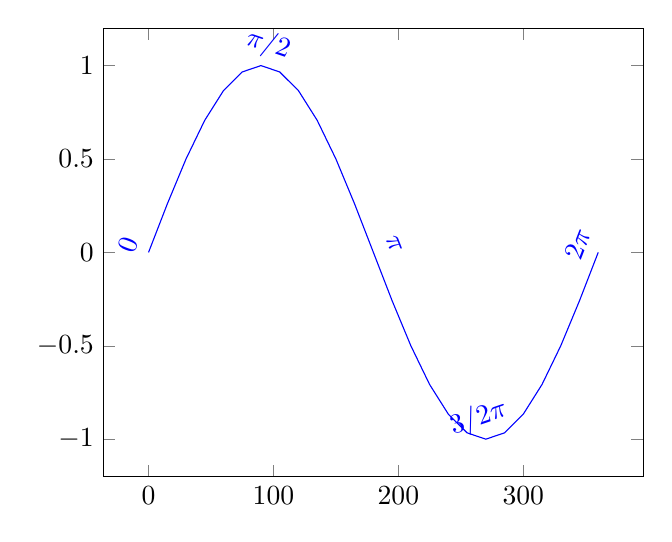
\begin{tikzpicture}
	\begin{axis}
	\addplot[blue,domain=0:360,samples=25] {sin(x)} 
	[every node/.style={yshift=8pt},sloped]
		node[pos=0] {$0$} 
		node[pos=0.25] {$\pi/2$}
		node[pos=0.5] {$\pi$}
		node[pos=0.75] {$3/2\pi$}
		node[pos=1] {$2\pi$}
	;
	\end{axis}
\end{tikzpicture}
\end{document}
